\section{Multiple Linear Regression}\label{sc:multipleLinearRegression}

\subsection{Theory}

Basic theory for simple and multiple lin regs here. From the slides or book\footnote{\cite{James2013}}.

Simple Linear Regression is used to make linear models of data. It has a response Y on the basis of a single predictor variable X. We can write it as:
\begin{align}\label{fo:simpleLinearRegression}
Y = \beta_0 + \beta_1 X_1 + \epsilon_i
\end{align}
$ \beta_0 + \beta_1 $ are unknown and to get a response, we must use data to estimate the coefficients.$(x_1, y_1)$, $(x_2, y_2)$,\ldots, $(x_n, y_n)$ represent n observation pairs, each of which consists of a measurement of X and a measurement of Y. The drawback of this method is that only a single predictor variable is used and often have more.
 In cases where we want examined the relationship between multiple predictor variables we use Multiple Linear Regression. The model takes the following form:
\begin{align}\label{fo:multipleLinearRegression}
Y = \beta_0 + \beta_1 X_1 + \ldots + \beta_n X_n + \epsilon_i
\end{align}
To obtain the estimated Coefficients in the model we use the least squares method to minimize the sum of squared residuals. We pick $\beta_0, \beta_1, ... \beta_p$ to to minimize the sum of squared residuals.
\begin{align}\label{fo:rss}
RSS = \sum (y - \hat{y})^2 = \sum( y_i - \hat{\beta_0} - \hat{\beta_1}x_{i1} - \hat{\beta_2}x_{i2} - \ldots - \hat{\beta_p}x_\textit{i}p )^2
\end{align}
To evaluated the model we can use RSE (residual standard error). This is done by meaning and rooting the result of the RSS. The outcome of the formula is the average amount that the response will deviate from the regression line. This is also known as an estimate of the $\epsilon$ in the Standard Linear Regression formula (\ref{fo:simpleLinearRegression}) stated earlier in this chapter:
\begin{align}\label{fo:rse}
RSE = \sqrt{\dfrac{1}{n-2}\cdot RSS}
\end{align}


\subsection{Results}
In lab 3.6.2 and 3.6.3 we use linear and multiple regression respectively, to test if there is a dependency between any of the values. The dataset tested on is housing values in suburbs of Boston\footnote{https://raw.github.com/vincentarelbundock/Rdatasets/master/csv/MASS/Boston.csv}.

\subsubsection*{LAB 3.6.2}
In this lab we make a linear regression on MEDV (\textit{Median value of owner-occupied homes in \$1000's}) and LSTAT (\textit{Lower status of the population}). Starting off by making a scatterplot of the data to observe how the data look compared to each other.

\begin{lstlisting}[language=Python]
sns.pairplot(data[['lstat','medv']],size=7)
plt.show()
\end{lstlisting}

\begin{figure}[h]
	\centering
	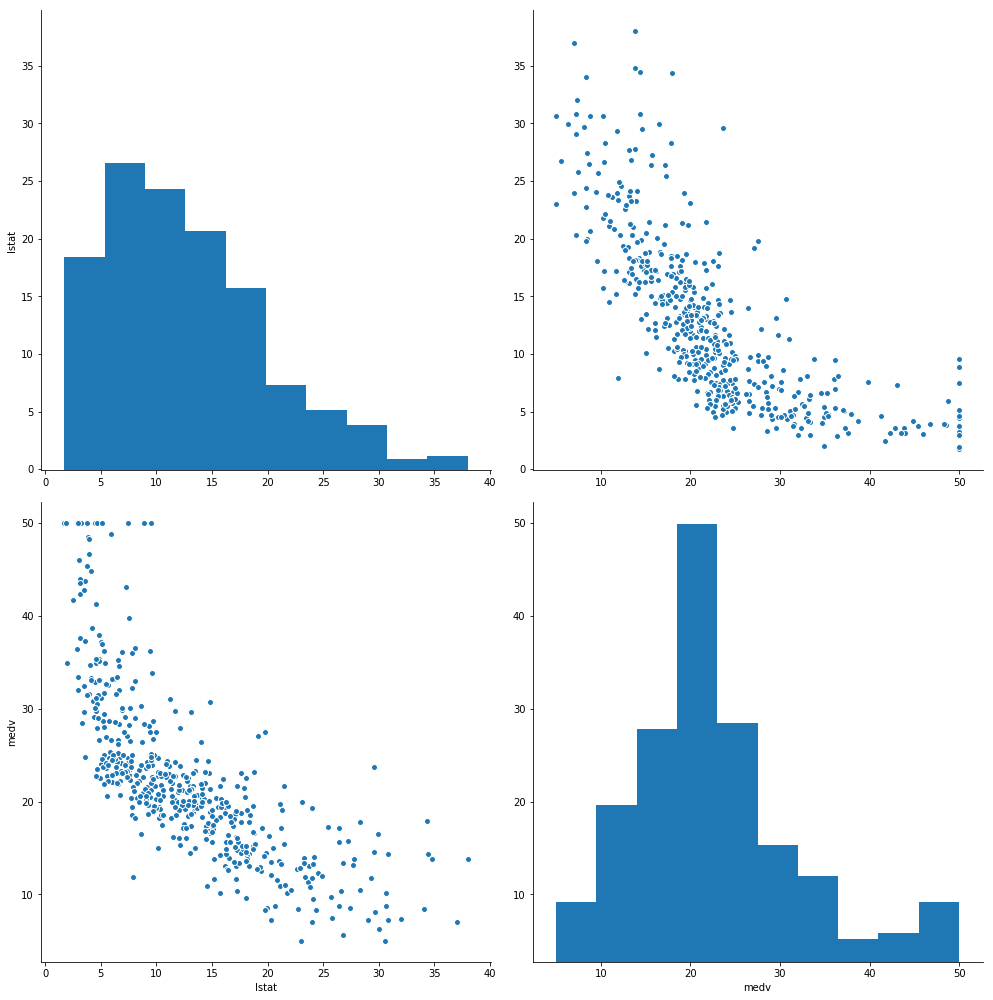
\includegraphics[scale=0.4, trim=0 0 0 500, clip=true]{regression/multipleLinearRegression/fig/bostonPairplotMdevLstat.png}
	\caption{Relationship between the feature and the response using scatterplots.}
	\label{fig:bostonPairplotMdevLstat}
\end{figure}

On Figure \ref{fig:bostonPairplotMdevLstat} we can already see that making a simple linear regression on these data, might be stretching it. Still we continue and try making a linear regression with the following lines of code.

\begin{lstlisting}[language=Python]
feature_cols = ['lstat']
X = data[feature_cols].values
y = data['medv'].values
from sklearn.linear_model import LinearRegression
linreg = LinearRegression()
linreg.fit(X, y)
print('Intercept: \n', linreg.intercept_)
print('Coefficients: \n', linreg.coef_)
y_pred = linreg.predict(X)
np.sqrt(metrics.mean_squared_error(y, y_pred))
print('Variance score: %.2f' % metrics.r2_score(y, y_pred))
\end{lstlisting}

Resulting in the following output:\\
\textit{Intercept: 34.5538408794\\
Coefficients: [-0.95004935]\\
Variance score: 0.54\\}

As we can see we have a variance score of 0.54, which tells us that the simple linear fit on these data isn't very precise. Making a scatterplot with the linear fit we can also visualize this observation.

\begin{figure}[h]
	\centering
	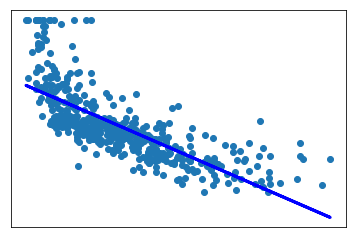
\includegraphics[scale=0.6]{regression/multipleLinearRegression/fig/bostonScatterplotMdevLstatLinreg.png}
	\caption{Relationship between the feature and the response using scatterplots, with linear fit.}
	\label{fig:bostonScatterplotMdevLstatLinreg}
\end{figure}

As we see on Figure \ref{fig:bostonScatterplotMdevLstatLinreg} both datapoints at the start and at the end is far away from the linear fit. We can conclude on both the variance and the observed data that there is some evidence of non-linearity.

\subsubsection*{LAB 3.6.3}
In this lab we continue working on the MDEV and LSTAT data, but also include AGE (\textit{proportion of owner-occupied units built prior to 1940}) to the mix in order for us to make multiple linear regressions on these datasets. Once again we start of making a scatterplot of the data in order for us to observe the datasets compared to each other. This time taking a step further and get an approximate of the linear regression fit, as seen on Figure \ref{fig:bostonPairplotMdevLstatAge}.

\begin{lstlisting}[language=Python]
sns.pairplot(data, x_vars=['lstat','age'], y_vars='medv', size=7, aspect=0.7, kind='reg')
plt.show()
\end{lstlisting}

\begin{figure}[h]
	\centering
	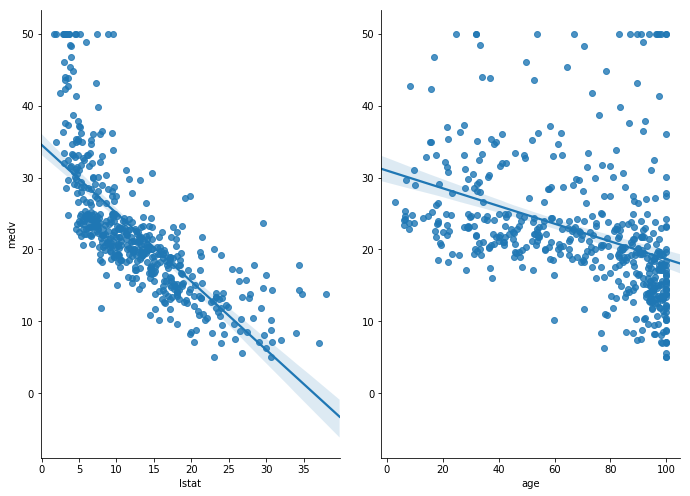
\includegraphics[scale=0.4]{regression/multipleLinearRegression/fig/bostonPairplotMdevLstatAge.png}
	\caption{Relationship between the feature and the response using scatterplots.}
	\label{fig:bostonPairplotMdevLstatAge}
\end{figure}

We then make a linear regression on the features and the response with the following lines of code.

\begin{lstlisting}[language=Python]
feature_cols = ['lstat','age']
X = data[feature_cols].values
y = data['medv'].values
linreg = LinearRegression()
linreg.fit(X, y)
print('Intercept: \n', linreg.intercept_)
print('Coefficients: \n', # pair the feature names with the coefficients
list(zip(feature_cols, linreg.coef_)))
y_pred = linreg.predict(X)
np.sqrt(metrics.mean_squared_error(y, y_pred))
print('Variance score: %.2f' % metrics.r2_score(y, y_pred))
\end{lstlisting}

Resulting in the following output:\\
\textit{Intercept: 33.2227605318\\
	Coefficients: [('lstat', -1.0320685641826013), ('age', 0.034544338571646085)]\\
	Variance score: 0.55\\}

Once again we can see that the variance score is too low for us to assume linearity and therefore we once again conclude that there is some evidence of non-linearity.

\subsection{Conclusion}
Linear regression is a good way of observing a dataset and checking if there is a linear or non-linear dependency between any of the data. However it is a very simple regression and because of this, often won't be able to give a high variance score, resulting in a high deviation from the fit.